%%%%%%%%%%%%%%%%%%%%%%%%%%%%%%%%%%%%%%%%%%%%%%%%%%%%%%%%%%%%%%%%%
%%% %
%%% % weiiszablon.tex
%%% % The Faculty of Electrical and Computer Engineering
%%% % Rzeszow University Of Technology diploma thesis Template
%%% % Szablon pracy dyplomowej Wydziału Elektrotechniki 
%%% % i Informatyki PRz
%%% % June, 2015
%%%%%%%%%%%%%%%%%%%%%%%%%%%%%%%%%%%%%%%%%%%%%%%%%%%%%%%%%%%%%%%%%

\documentclass[12pt,twoside]{article}

\usepackage{weiiszablon}
\usepackage{csquotes}
\usepackage{float}

\author{Łukasz Miłoś}

% np. EF-123456, EN-654321, ...
\studentID{EF-161883}

\title{System zarządzania bazą BOM}

%%% wybierz rodzaj pracy wpisując jeden z poniższych numerów: ...
% 1 = inżynierska	% BSc
% 2 = magisterska	% MSc
% 3 = doktorska		% PhD
%%% na miejsce zera w linijce poniżej
\newcommand{\rodzajPracyNo}{0}

%%% promotor
\supervisor{(dr inż.) Mariusz Borkowski (prof. PRz)}
%% przykład: dr hab. inż. Józef Nowak, prof. PRz

%%% promotor ze stopniami naukowymi po angielsku
\supervisorEN{(EngD) Mariusz Borkowski}

\begin{document}

% strona tytułowa
\maketitle
\blankpage

% spis treści
\tableofcontents
\clearpage
\blankpage

\section{Wstęp}
Projekt dotyczy przedmiotu \enquote{Usługi sieciowe w biznesie} i zgodnie z założeniami ma ściśle praktyczny charakter.

Sam przedmiot skupia się na zagadnieniach informatyzacji w przedsiębiorstwach, które wpływają na ich organizację i strukturę. Dzięki zastosowaniu różnej klasy systemów, działania ludzkie są wspierane, a często także zastępowane poprzez wykorzystanie nowych technologii, co ma swoje odzwierciedlenie w większej wydajności, produktywności, mniejszym ryzyku popełnienia błędu, a co za tym idzie także minimalizacji kosztów operacyjnych. Wiele zagadnień w przedsiębiorstwach można ułatwić poprzez zastosowanie odpowiedniego systemu zintegrowanego, stąd niezbędna wiedza o typach, funkcjach i przypadkach użycia poszczególnych technologii.

Spośród mnogości zagadnień wybrano temat dotyczący organizacji zasobów produkcyjnych, jako bardzo istotny element wielu przedsiębiorstw.

W ramach projektu utworzono system zarządzania bazą BOM (Bill of Materials). Zagadnienie to jest ściśle związane z przedmiotem i zostanie opisane w kolejnym rozdziale.

\clearpage

\section{Opis problemu}

BOM (Bill Of Materials) jest strukturalnym (hierarchicznym) zestawieniem materiałowym produktu końcowego zawierającym listę części składowych niezbędnych do jego wytworzenia wraz z podaniem cech określających dany zasób m.in. ceny i ilości. Takie zestawienia są wykorzystywane na różnych etapach produkcji, zarówno podczas projektowania, a także podczas wytwarzania czy nawet montażu.

Niekiedy BOM jest wzbogacany o opis kolejnych czynności, w których używane są poszczególne elementy składowe (przykładem jest dowolna instrukcja szafy przeznaczonej do samodzielnego montażu, która często zawiera elementy składowe wraz z wyszczególnieniem kolejnych czynności montażowych).

Poszczególne elementy posiadają kilka cech (atrybutów). W zależności od implementacji systemu parametry są różne. Oto kilka najpopularniejszych z nich:

\begin{itemize}[label=-,labelsep=0.4cm,leftmargin=0.6cm]
\item nazwa
\item identyfikator
\item ilość
\item jednostka miary
\item cena jednostkowa
\item cena sumaryczna
\end{itemize}

Wyjściowym etapem w konstrukcji zestawienia materiałowego może być ogólne, koncepcyjne przedstawienie części składowych produktu finalnego w formie rysunku (\ref{fig:example:drawing}) lub grafu (\ref{fig:example:graph}).

\begin{figure}
	\centering
	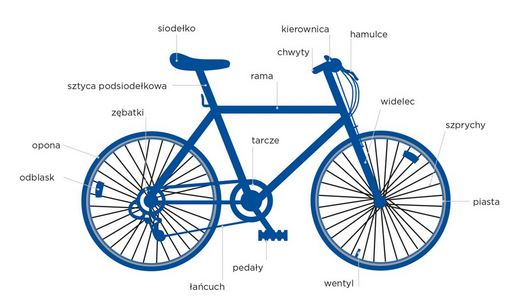
\includegraphics[width=\textwidth]{figures/examples/drawing.jpg}
	\caption{Przykład koncepcyjnego zestawienia BOM w formie rysunku [https://www.mecalux.pl/blog/zestawienie-materialowe-bom]}
\label{fig:example:drawing}
\end{figure}

Należy zwrócić uwagę, że poszczególne elementy składowe, także składają się z mniejszych komponentów (hierarchia). Ważne jest zaprezentowanie odpowiedniego stopnia złożoności, który zależy od specyfiki danego przedsiębiorstwa. Przykładowo dla firmy produkującej rowery, schemat (\ref{fig:example:drawing}) może okazać się wystarczający, jeśli korzysta ona z gotowych produktów innych firm, a nie tworzy wszystkiego na własną rękę. Przykładem jest tutaj półprodukt hamulca. O ile firma zakupuje gotowe hamulce od innej marki i tylko montuje je w swoich rowerach to ten poziom wyszczególnienia jest wystarczający. Natomiast w przypadku produkcji hamulców na wewnętrznie, należałoby dodatkowo wyszczególnić części składowe hamulca (m.in. rączkę, mocowanie, śruby mocujące, linkę, gumki ścieralne, gumki ochronne, smar itd.).

Innym sposobem koncepcyjnego zapisu zestawienia materiałowego dowolnego produktu może być graf(\ref{fig:example:graph}). Na podstawie grafu można przedstawić hierarchię, ale nie jest możliwe przedstawienie informacji szczegółowych dotyczących poszczególnych wyrobów.

\begin{figure}
	\centering
	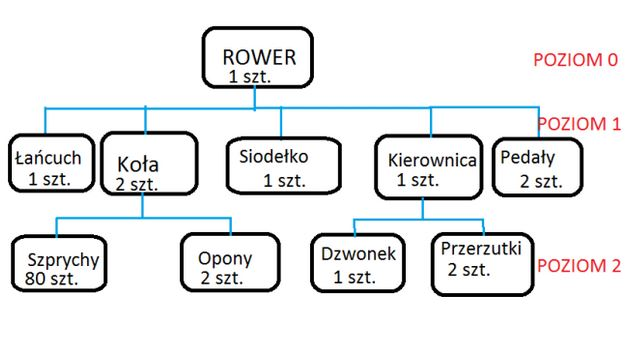
\includegraphics[width=\textwidth]{figures/examples/graph.jpg}
	\caption{Przykład koncepcyjnego zestawienia BOM w formie grafu [https://logistykanalogike.wordpress.com/2014/12/18/struktura-wyrobu/]}
\label{fig:example:graph}
\end{figure}

W rzeczywistości zestawienia materiałowe przyjmują jednak formę hierarchii (\ref{fig:example:hierarchy}) lub tabeli (\ref{fig:example:table}), z wyszczególnieniem poszczególnych elementów składowych.

\begin{figure}
	\centering
	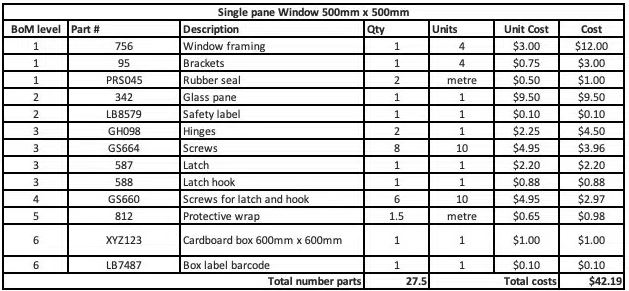
\includegraphics[width=\textwidth]{figures/examples/table.jpg}
	\caption{Przykład zestawienia BOM w formie tabeli [https://www.unleashedsoftware.com/blog/everything-you-need-to-know-about-bill-of-materials]}
\label{fig:example:table}
\end{figure}

Niestety wykorzystanie tabeli nie przedstawia wprost hierarchii poszczególnych komponentów. Hierarchia jest tutaj (\ref{fig:example:table}) oznaczona za pomocą pierwszej kolumny (BoM level). Zestawienie w formie tabeli w tym przypadku zawiera identyfikator części, opis, ilość, jednostkę, koszt jednostkowy i koszt całościowy. Warto także zwrócić uwagę na podsumowanie zawierające sumę ilości poszczególnych części, a także sumę kosztów.

Najlepszym sposobem prezentacji zestawienia materiałowego (BOM) jest pokazanie hierarchii (\ref{fig:example:hierarchy}), np. za pomocą drzewa hierachicznego (treeview).

\begin{figure}2
	\centering
	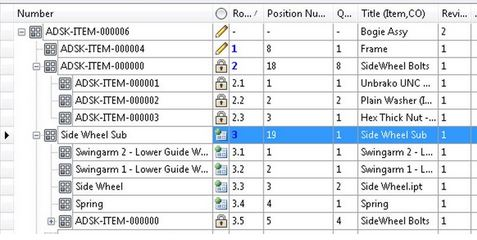
\includegraphics[width=\textwidth]{figures/examples/hierarchy.jpg}
	\caption{Przykład zestawienia BOM w formie drzewa hierarchicznego [https://underthehood-autodesk.typepad.com/blog/items/page/2/]}
\label{fig:example:hierarchy}
\end{figure}

Na załączonym zdjęciu (\ref{fig:example:hierarchy}) pokazano przykład docelowej hierarchii. Jest także możliwość rozwijania i zwijania poszczególnych elementów składowych, co pozwala zwiększyć czytelność zestawienia.

Temat organizacji zasobów produkcyjnych jest bardzo istotny, ponieważ umożliwia zachowanie ciągłości produkcji, a także pozwala na utrzymanie płynności finansowej przedsiębiorstwa.

Dzięki posiadaniu precyzyjnych zestawień można planować zakup surowców (ustrzeżenie się braku, ale także nadmiaru zapasów), a także określać niezbędne do poniesienia koszty (planowanie budżetu). Nie można również zapomnieć o tym, że mając wiedzę na temat niezbędnych materiałów i ich ilości można zarządzać zapasami na przyszłość i nie dopuścić do braku materiałów w magazynie, co jest bardzo niebezpieczne. Istotny jest także atut minimalizacji błędów, zyskany dzięki korzystaniu z utworzonego zestawienia.

Projekt jest zatem próbą znalezienia rozwiązania poprzez utworzenie własnego systemu do zarządzania hierarchiczną bazą BOM. Naturalnie takie systemy istnieją na rynku, ale są one zazwyczaj częścią zintegrowanych systemów zarządzania przedsiębiorstwem i nie stanowią oddzielnych bytów.

\clearpage
\section{Rozwiązanie}

\subsection*{Zalecenia}
Analiza problemu doprowadziła do powstania pewnych zaleceń implementowanego systemu. Celem jest wykorzystanie zalet innych systemów, a także eliminacja ich wad. Najważniejsze zalecenia spisano poniżej:

\begin{itemize}[label=-,labelsep=0.4cm,leftmargin=0.6cm]
\item system ma być prosty i niezależny od innego oprogramowania (samodzielny)
\item bardzo istotna jest prezentacja zestawienia materiałowego w postaci hierarchii, a także pokazanie szczegółów poszczególnych wyrobów. 
\item program powinien posiadać wygodny i intuicyjny interfejs użytkownika
\item możliwość dodawania, usuwania i edycji poszczególnych pozycji zestawienia
\end{itemize}

\subsection*{Założenia}
Na podstawie założeń zdecydowano się na implementację systemu przy użyciu języka programowania Python i wbudowanej biblioteki do obsługi interfejsu graficznego o nazwie tkinter. Python został wybrany jako  przyszłościowy język wysokiego poziomu o wielorakich zastosowaniach. Biblioteka graficzna ułatwia proces tworzenia interfejsu graficznego i pozwala się skupić na faktycznej realizacji. Przy pomocy tych dwóch narzędzi można zorganizować niemal cały wymagany system.

Istotnym zagadnieniem jest jednak przechowywanie danych, ponieważ bez tego zestawienie istniałoby tylko podczas działania programu (przechowywane w pamięci). W celu uzyskania pełnej niezależności postawiono na przechowywanie zestawień w lokalnych plikach komputera w formacie JSON. Jest to tekstowy format zapisu danych, który już sam w sobie jest hierarchiczny.

\clearpage
\section{Przykłady użycia}

\clearpage
\section{Podsumowanie}

\clearpage

\addcontentsline{toc}{section}{Literatura}
\begin{thebibliography}{8}
\label{sec:bibliography}
https://www.mecalux.pl/blog/zestawienie-materialowe-bom
https://www.system-kanban.pl/definicja/bom-bill-of-materials/
https://www.unleashedsoftware.com/blog/everything-you-need-to-know-about-bill-of-materials
\end{thebibliography}
\clearpage

\end{document} 
